\section[pbdDMAT eg's]{Examples Using pbdDMAT}
\setcounter{excount}{0}


\hidenum
\begin{frame}[noframenumbering]
\frametitle{Contents}
 \tableofcontents[currentsection,hideothersubsections,sectionstyle=show/hide]
\end{frame}
\shownum

% 
% 
% \subsection{Manipulating DMAT Objects}
% 
% \begin{frame}[fragile,shrink]
%   \begin{exampleblock}{Example \countex:  DMAT Construction}\pause
% \begin{lstlisting}[title=Generate a global matrix and distribute it]
% library(pbdDMAT, quiet=TRUE)
% init.grid()
% 
% # Common global on all processors --> distributed
% x <- matrix(1:100, nrow=10, ncol=10)
% x.dmat <- as.ddmatrix(x)
% 
% x.dmat
% 
% # Global on processor 0 --> distributed
% if (comm.rank()==0){
%   y <- matrix(1:100, nrow=10, ncol=10)
% } else {
%   y <- NULL
% }
% y.dmat <- as.ddmatrix(y)
% 
% y.dmat
% 
% finalize()
% \end{lstlisting}
% \begin{lstlisting}[basicstyle=\tiny,backgroundcolor=\color{white},keywordstyle=\color{black},title=\fontsize{6pt}{7.2}\selectfont Execute this script via:]
% mpirun -np 2 Rscript 1_gen.r
% \end{lstlisting} 
%   \end{exampleblock}
% \end{frame}
% 
% 
% 
% \begin{frame}[fragile]
%   \begin{exampleblock}{Example \countex:  DMAT Construction}\pause
% \begin{lstlisting}[title=Generate locally only what is needed]
% library(pbdDMAT, quiet=TRUE)
% init.grid()
% 
% zero.dmat <- ddmatrix(0, nrow=100, ncol=100)
% zero.dmat
% 
% id.dmat <- diag(1, nrow=100, ncol=100, type="ddmatrix")
% id.dmat
% 
% comm.set.seed(diff=T)
% rand.dmat <- ddmatrix("rnorm", nrow=100, ncol=100, mean=10, sd=100)
% rand.dmat
% 
% finalize()
% \end{lstlisting}
% \begin{lstlisting}[basicstyle=\tiny,backgroundcolor=\color{white},keywordstyle=\color{black},title=\fontsize{6pt}{7.2}\selectfont Execute this script via:]
% mpirun -np 2 Rscript 2_gen.r
% \end{lstlisting} 
%   \end{exampleblock}
% \end{frame}
% 
% 
% \begin{frame}[fragile]
%   \begin{exampleblock}{Example \countex:  DMAT Operations}\pause
% \begin{lstlisting}[title=Generate locally only what is needed]
% library(pbdDMAT, quiet=TRUE)
% init.grid()
% 
% x.dmat <- ddmatrix(1:30, nrow=10)
% y.dmat <- x.dmat[c(1, 3, 5, 7, 9), -3]
% 
% comm.print(y.dmat)
% y <- as.matrix(y.dmat)
% comm.print(y)
% 
% finalize()
% \end{lstlisting}
% \begin{lstlisting}[basicstyle=\tiny,backgroundcolor=\color{white},keywordstyle=\color{black},title=\fontsize{6pt}{7.2}\selectfont Execute this script via:]
% mpirun -np 2 Rscript 3_extract.r
% \end{lstlisting} 
%   \end{exampleblock}
% \end{frame}
% 
% 
% 
% \begin{frame}[fragile]
%   \begin{exampleblock}{Example \countex:  More DMAT Operations}\pause
% \begin{lstlisting}
% library(pbdDMAT, quiet=TRUE)
% init.grid()
% 
% x.dmat <- ddmatrix(1:30, nrow=10)
% 
% y.dmat <- x.dmat + 1:7
% 
% z.dmat <- scale(x.dmat, center=TRUE, scale=TRUE)
% 
% y <- as.matrix(y.dmat)
% z <- as.matrix(z.dmat)
% 
% comm.print(y)
% comm.print(z)
% 
% finalize()
% \end{lstlisting}
% \begin{lstlisting}[basicstyle=\tiny,backgroundcolor=\color{white},keywordstyle=\color{black},title=\fontsize{6pt}{7.2}\selectfont Execute this script via:]
% mpirun -np 2 Rscript 4_misc.r
% \end{lstlisting} 
%   \end{exampleblock}
% \end{frame}
% 
% 


% \begin{frame}[fragile]
%   \begin{exampleblock}{Example \countex:  GBD and DMAT}\pause
% \begin{lstlisting}
% library(pbdDEMO, quiet=TRUE)
% init.grid()
% 
% comm.set.seed(diff = TRUE)
% 
% N.gbd <- 1 + comm.rank()
% X.gbd <- matrix(rnorm(N.gbd * 3), ncol = 3)
% 
% # convert GBD to DMAT
% X.dmat <- gbd2dmat(X.gbd)
% 
% # convert DMAT to GBD
% new.X.gbd <- dmat2gbd(X.dmat)
% 
% # undistribute
% X <- as.matrix(X.dmat)
% 
% finalize()
% \end{lstlisting}
% \begin{lstlisting}[basicstyle=\tiny,backgroundcolor=\color{white},keywordstyle=\color{black},title=\fontsize{6pt}{7.2}\selectfont Execute this script via:]
% mpirun -np 2 Rscript 4_convert.r
% \end{lstlisting} 
%   \end{exampleblock}
% \end{frame}



\subsection{Statistics Examples with pbdDMAT}

\begin{frame}[fragile]
  \begin{exampleblock}{Sample Covariance}\pause
\begin{lstlisting}[title=Serial Code]
Cov.X <- cov(X)
print(Cov.X)
\end{lstlisting}

\begin{lstlisting}[title=Parallel Code]
Cov.X <- cov(X)
print(Cov.X)
\end{lstlisting}
  \end{exampleblock}
\end{frame}

\begin{frame}[fragile,shrink]
  \begin{exampleblock}{Linear Regression}\pause
\begin{lstlisting}[title=Serial Code]
tX <- t(X)
A <- tX %*% X
B <- tX %*% y

ols <- solve(A) %*% B

# or
ols <- lm.fit(X, y)
\end{lstlisting}
  
\begin{lstlisting}[title=Parallel Code]
tX <- t(X)
A <- tX %*% X
B <- tX %*% y

ols <- solve(A) %*% B

# or
ols <- lm.fit(X, y)
\end{lstlisting}
  \end{exampleblock}
\end{frame}



\begin{frame}[fragile]
\fontsize{8pt}{7.2}\selectfont
  \begin{exampleblock}{Example 5:  PCA}
\begin{lstlisting}[basicstyle=\tiny,title=\fontsize{8pt}{7.2}\selectfont PCA: pca.r]
library(pbdDMAT, quiet=T)
init.grid()

n <- 1e4
p <- 250

comm.set.seed(diff=T)
x.dmat <- ddmatrix("rnorm", nrow=n, ncol=p, mean=100, sd=25)

pca <- prcomp(x=x.dmat, retx=TRUE, scale=TRUE)
prop_var <- cumsum(pca$sdev)/sum(pca$sdev)
i <- max(min(which(prop_var > 0.9)) - 1, 1)

y.dmat <- pca$x[, 1:i]

comm.cat("\nCols: ", i, "\n", quiet=T)
comm.cat("%Cols:", i/dim(x.dmat)[2], "\n\n", quiet=T)

finalize()
\end{lstlisting}
\vspace{-.4cm}
  \begin{columns}[t,onlytextwidth]
    \begin{column}{0.58\textwidth}
\begin{lstlisting}[basicstyle=\tiny,backgroundcolor=\color{white},keywordstyle=\color{black},title=\fontsize{6pt}{7.2}\selectfont Execute this script via:]
mpirun -np 2 Rscript 5_pca.r
\end{lstlisting}    
    \end{column}
    \hfill
    \begin{column}{0.4\textwidth}
\begin{lstlisting}[basicstyle=\tiny,title=\fontsize{6pt}{7.2}\selectfont Sample Output:]
Cols:  221 
%Cols: 0.884 
\end{lstlisting}
    \end{column}
​  \end{columns}
  \end{exampleblock}
\end{frame}



\begin{frame}
  \begin{block}{Distributed Matrices}\pause
  \begin{center}
    \pkg{pbdDEMO} contains many other examples of reading and managing GBD and DMAT data
  \end{center}
  \end{block}
\end{frame}



% \begin{frame}
%  \fontsize{8pt}{10}\selectfont
%   \begin{block}{Randomized SVD Algorithm\footnotemark}\pause
% Given an $m\times n$ matrix $\bs{A}$, a target number $k$ of singular 
% vectors, and an exponent $q$ (say, $q=1$ or $q=2$), this procedure computes an 
% approximate rank-$2k$ factorization $\bs{U}\bs{\Sigma}\bs{V}^*$, where $\bs{U}$ 
% and $\bs{V}$ are 
% orthonormal, and $\bs{\Sigma}$ is nonnegative and diagonal.\\[.2cm]
% \textbf{Stage A:}
% \begin{enumerate}
%   \item Generate an $n\times 2k$ Gaussian test matrix $\bs{\Omega}$.
%   \item Form $\bs{Y}_0 = \bs{A}\bs{\Omega}$ and compute its QR factorization 
% $\bs{Y}_0 = \bs{Q}_0\bs{R}_0$
%   \item \textbf{for} $j = 1, 2, \dots, q$\\
%   \hspace{.4cm} Form $\bs{\widetilde{Y}}_j = \bs{A}^*\bs{Q}_{j-1}$ and compute 
% its QR factorization $\bs{\widetilde{Y}}_j = \bs{\widetilde{Q}}_j 
% \bs{\widetilde{R}}_j$\\
%   \hspace{.4cm} Form $\bs{Y}_j = \bs{A}\bs{\widetilde{Q}}_j$ and compute its QR 
% factorization $\bs{Y}_j = \bs{Q}_j \bs{R}_j$.\\
%   \textbf{end}
%   \item Let $\bs{Q} = \bs{Q}_q$, so that the columns of $\bs{Q}$ form an 
% orthonormal basis for the range of $\bs{Y}$.
% \end{enumerate}
% \textbf{Stage B:}
% \begin{enumerate}
%   \setcounter{enumi}{4}
%   \item Form $\bs{B} = \bs{Q}^* \bs{A}$
%   \item Compute an SVD of the small matrix: 
%   $\bs{B} = \bs{\widetilde{U}} \bs{\Sigma} \bs{V}^*$
%   \item Set $\bs{U} = \bs{Q}\bs{\widetilde{U}}$.
% \end{enumerate}
%   \footnotetext{ \fontsize{6pt}{10}\selectfont $^1$Halko N, Martinsson P-G 
% and Tropp J A 2011 Finding structure with randomness: probabilistic algorithms 
% for constructing approximate matrix decompositions \emph{SIAM} Rev. \textbf{53} 
% 217--88}
%   \end{block}
% \end{frame}

\subsection{RandSVD}

\begin{frame}[fragile]
\fontsize{8pt}{10}\selectfont
\begin{block}{Randomized SVD\footnotemark}
  \begin{minipage}{.55\textwidth}
    \begin{center}
      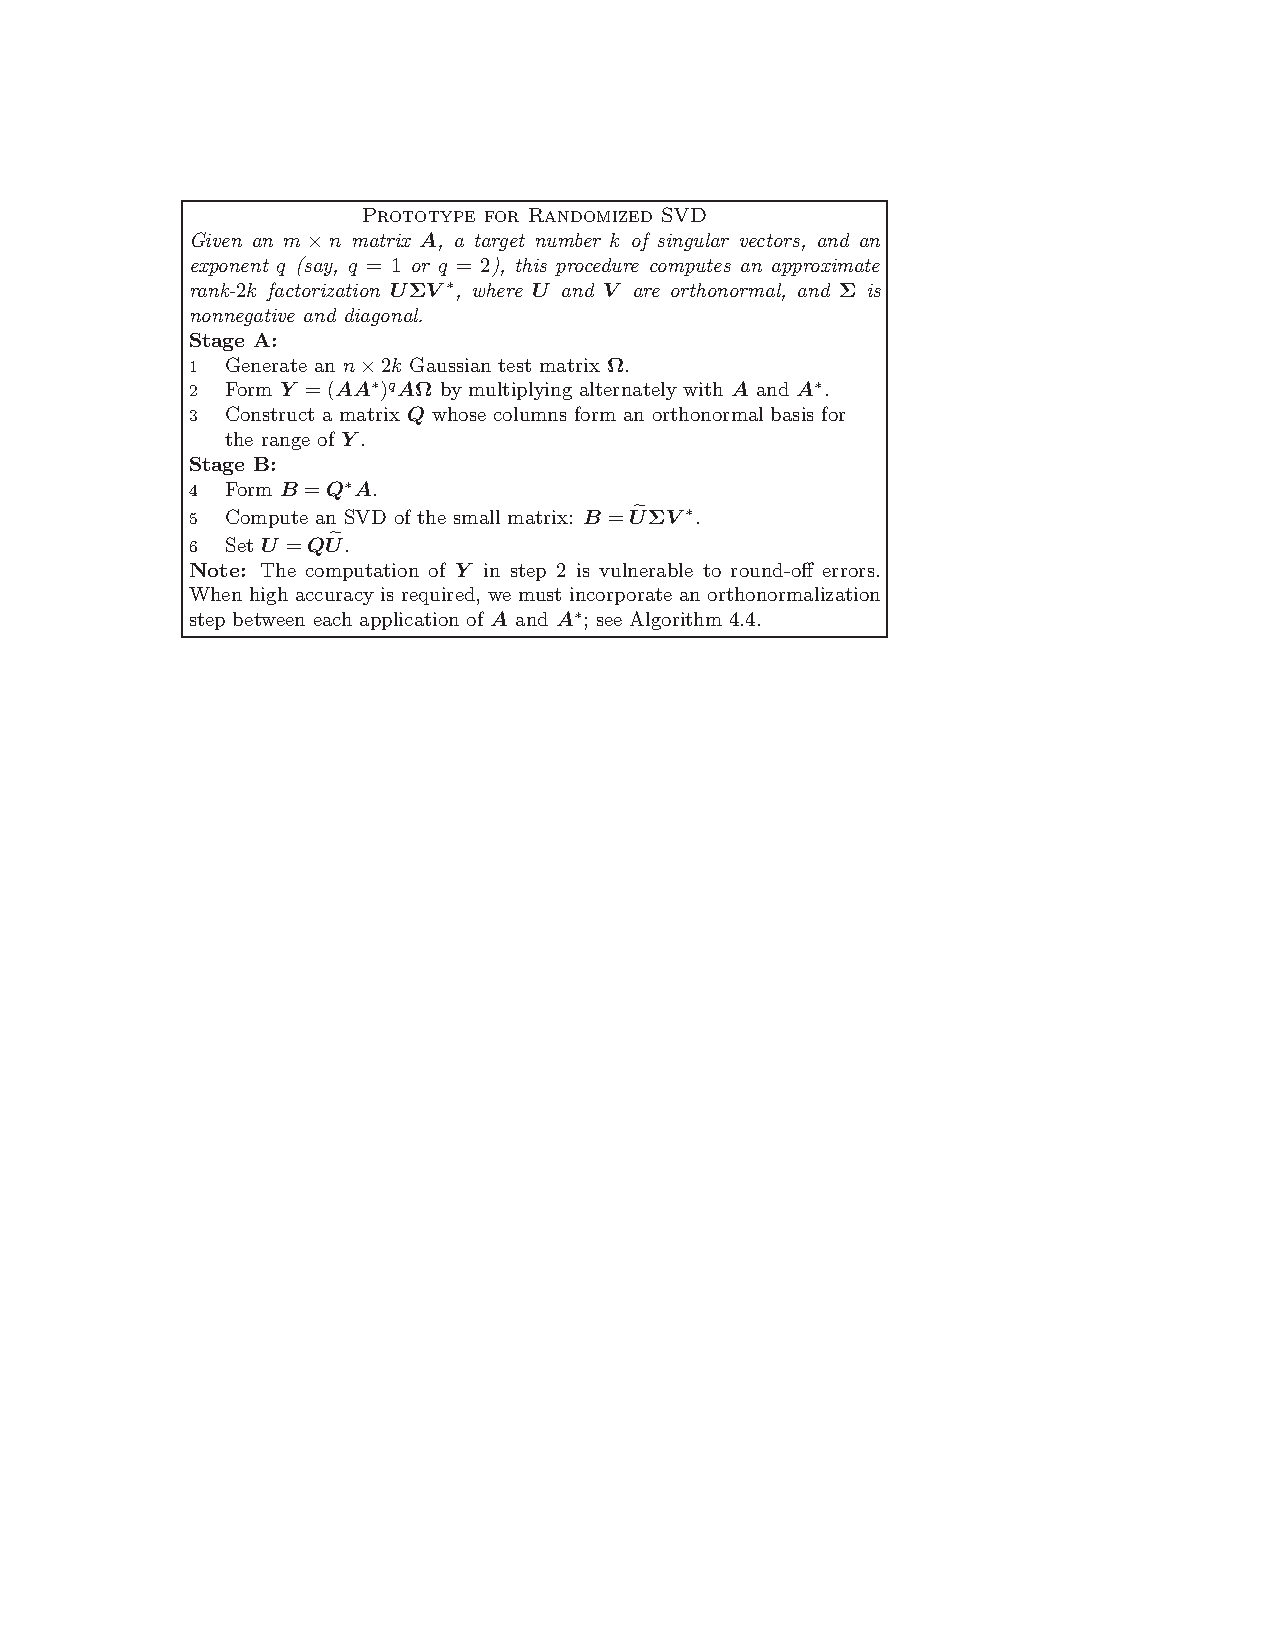
\includegraphics[width=.95\textwidth]{../common/pics/randSVDalg}
      \\
      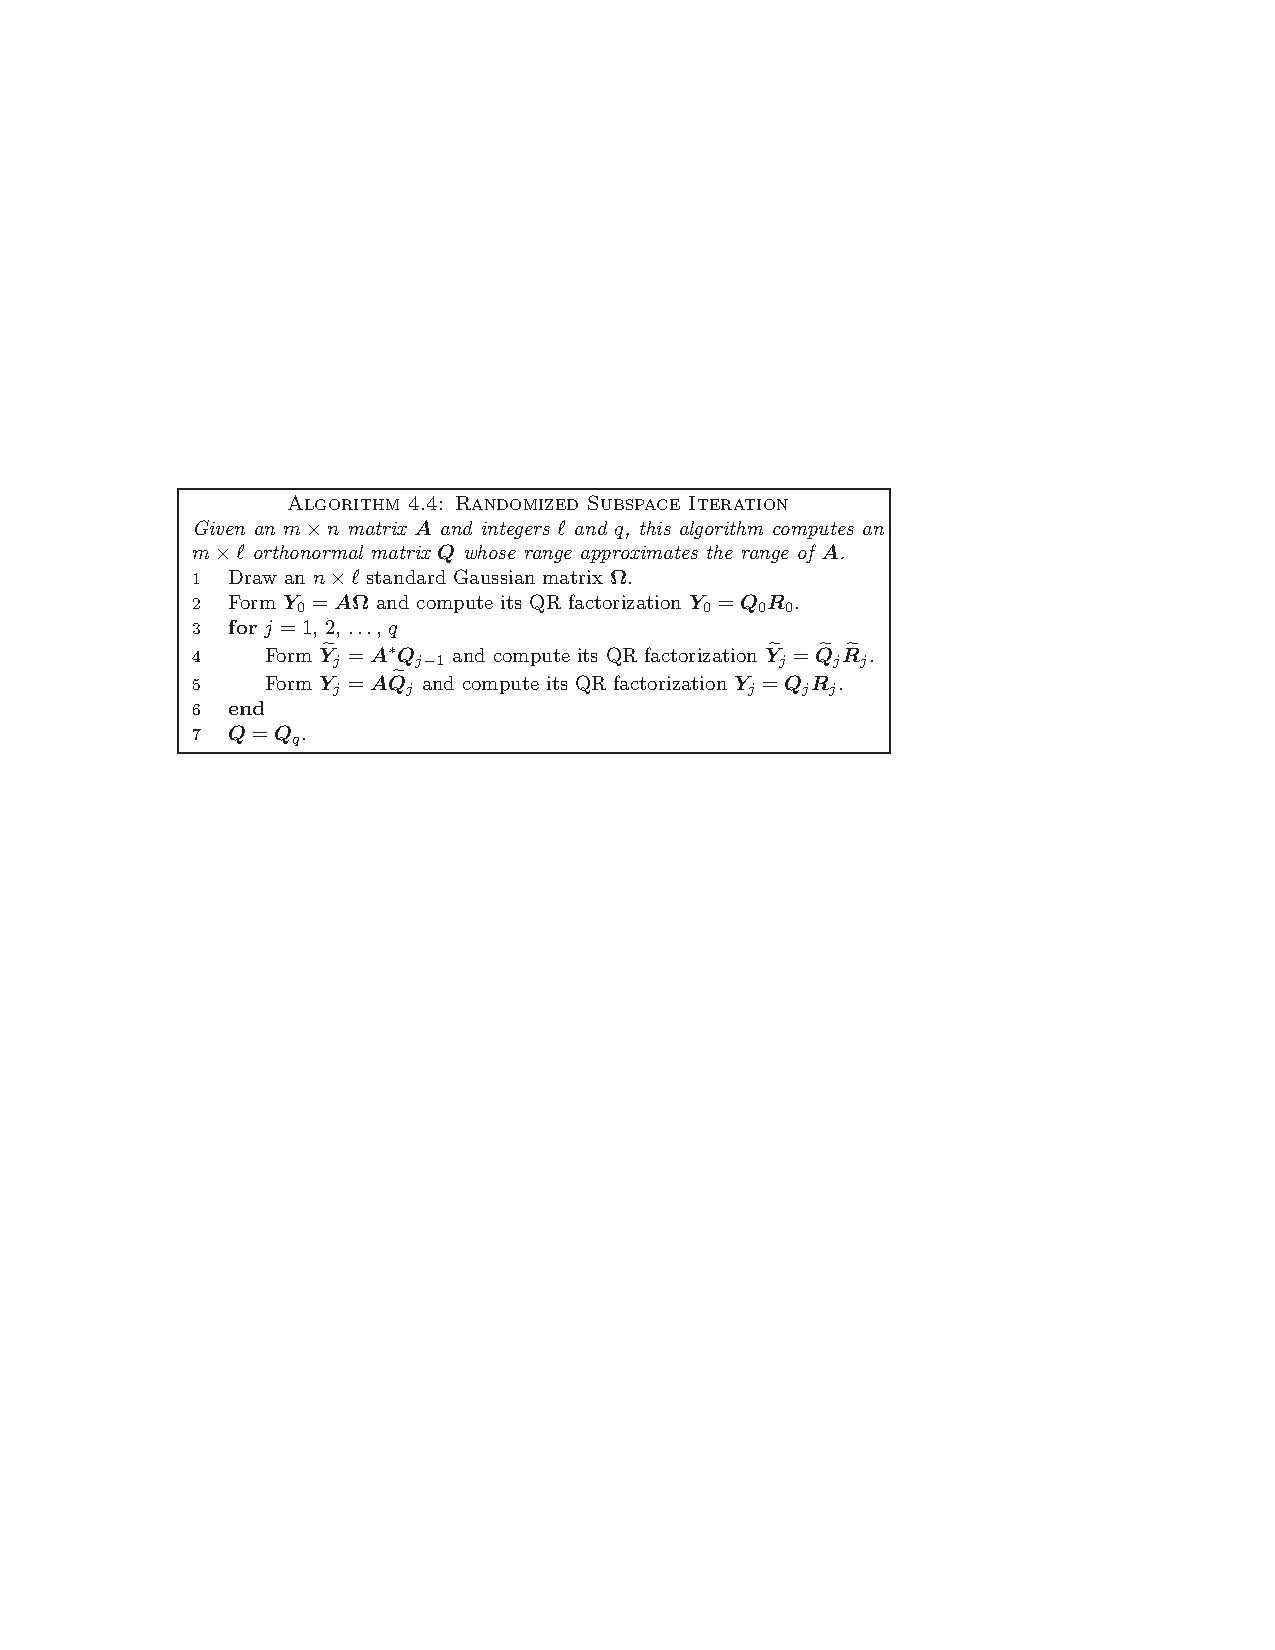
\includegraphics[width=.95\textwidth]{../common/pics/randSVDalg4_4}
    \end{center}
  \end{minipage}
%   \hspace{.01cm}
  \begin{minipage}{0.430\textwidth}
\begin{lstlisting}[title=Serial 
R,basicstyle=\tiny,backgroundcolor=\color{grayish} 
,numberstyle=\tiny\color{black},keywordstyle=\color{black},commentstyle=\color{ 
dkgreen},stringstyle=\color{black},escapeinside={(*@}{@*)}]
randSVD <- function(A, k, q=3)
  {
    ## Stage A
    Omega <- (*@ matrix(rnorm(n*2*k),@*) 
            (*@ nrow=n, ncol=2*k) @*)
    Y <- A %*% Omega
    Q <- qr.Q(qr(Y))
    At <- t(A)
    for(i in 1:q)
      {
        Y <- At %*% Q
        Q <- qr.Q(qr(Y))
        Y <- A %*% Q
        Q <- qr.Q(qr(Y))
      }
    
    ## Stage B
    B <- t(Q) %*% A
    U <- La.svd(B)$u
    U <- Q %*% U
    U[, 1:k]
  }
\end{lstlisting} %balance$
\end{minipage}
{\fontsize{6pt}{10}\selectfont $^1$Halko N, Martinsson P-G 
  and Tropp J A 2011 Finding structure with randomness: probabilistic algorithms 
  for constructing approximate matrix decompositions \emph{SIAM Rev.} \textbf{53} 
  217--88}
\end{block}
\end{frame}


\begin{frame}[fragile]
 \fontsize{8pt}{10}\selectfont
\begin{block}{Randomized SVD}
  \hfill
  \begin{minipage}{0.430\textwidth}
\begin{lstlisting}[title=Serial 
R,basicstyle=\tiny,backgroundcolor=\color{grayish} 
,numberstyle=\tiny\color{black},keywordstyle=\color{black},commentstyle=\color{ 
dkgreen},stringstyle=\color{black},escapeinside={(*@}{@*)}]
randSVD <- function(A, k, q=3)
  {
    ## Stage A
    Omega <- (*@ \textcolor{blue}{matrix(rnorm(n*2*k),} @*) 
         (*@ \textcolor{blue}{ nrow=n, ncol=2*k)} @*)
    Y <- A %*% Omega
    Q <- qr.Q(qr(Y))
    At <- t(A)
    for(i in 1:q)
      {
        Y <- At %*% Q
        Q <- qr.Q(qr(Y))
        Y <- A %*% Q
        Q <- qr.Q(qr(Y))
      }
    
    ## Stage B
    B <- t(Q) %*% A
    U <- La.svd(B)$u
    U <- Q %*% U
    U[, 1:k]
  }
\end{lstlisting} %balance$
  \end{minipage}
  \hfill
  \begin{minipage}{0.430\textwidth}
\begin{lstlisting}[title=Parallel pbdR,basicstyle=\tiny,backgroundcolor=\color{
grayish}, numberstyle=\tiny\color{black},keywordstyle=\color{black},
commentstyle=\color{dkgreen},stringstyle=\color{black},escapeinside={(*@}{@*)}]
randSVD <- function(A, k, q=3)
  {
    ## Stage A
    Omega <- (*@ \textcolor{blue}{ddmatrix("rnorm",} @*)
         (*@ \textcolor{blue}{nrow=n, ncol=2*k)} @*)
    Y <- A %*% Omega
    Q <- qr.Q(qr(Y))
    At <- t(A)      
    for(i in 1:q)
      {
        Y <- At %*% Q   
        Q <- qr.Q(qr(Y))
        Y <- A %*% Q    
        Q <- qr.Q(qr(Y))
      }
    
    ## Stage B
    B <- t(Q) %*% A     
    U <- La.svd(B)$u 
    U <- Q %*% U     
    U[, 1:k]
  }
\end{lstlisting}  % balancing $
  \end{minipage}
\hfill
\end{block}
\end{frame}

\begin{frame}
  \begin{block}{Randomized SVD}
    \begin{center}
      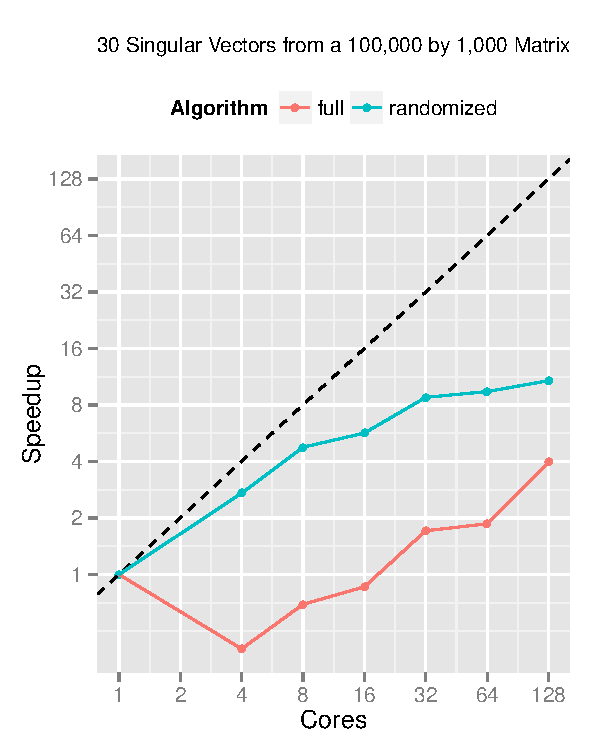
\includegraphics[width=.45\textwidth]{../common/pics/randSVDspeedup}
      \hfill
      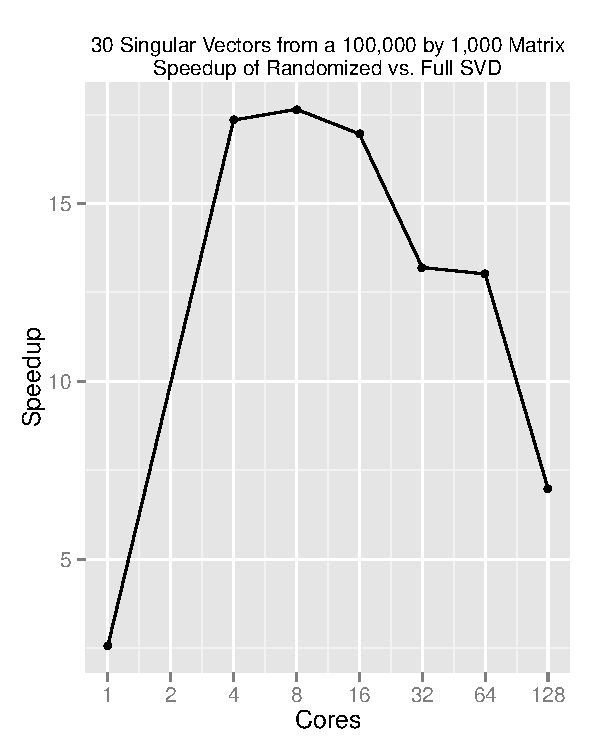
\includegraphics[width=.45\textwidth]{../common/pics/randSpeedupSVD}
    \end{center}
  \end{block}
\end{frame}